\documentclass[sigconf]{acmart}

\usepackage{booktabs} % For formal tables
\usepackage{amsmath}
\usepackage{graphicx,xspace,verbatim,comment}
\usepackage{hyperref,array,color,balance,multirow}
\usepackage{balance,float,url,amsfonts,alltt}
\usepackage{mathtools,rotating,amsmath,amssymb}
\usepackage{color,ifpdf,fancyvrb,array}
% \usepackage{algorithm,algpseudocode}
\usepackage{etoolbox,listings,subcaption}
\usepackage{bigstrut,morefloats}
%\usepackage[linesnumbered,boxruled]{algorithm2e}
\usepackage[boxruled]{algorithm2e}
\usepackage{pbox}

\DeclarePairedDelimiter{\ceil}{\lceil}{\rceil}
\DeclarePairedDelimiter{\floor}{\lfloor}{\rfloor}

\newcommand{\eat}[1]{}

\newenvironment{packeditems}{
\begin{itemize}
  \setlength{\itemsep}{1pt}
  \setlength{\parskip}{0pt}
  \setlength{\parsep}{0pt}
}{\end{itemize}}

\newenvironment{packedenums}{
\begin{enumerate}
  \setlength{\itemsep}{1pt}
  \setlength{\parskip}{0pt}
  \setlength{\parsep}{0pt}
}{\end{enumerate}}

\setcopyright{acmcopyright}
% \setcopyright{rightsretained}

\acmDOI{10.475/123_4}
\acmISBN{123-4567-24-567/08/06}
\acmConference[WOODSTOCK'97]{ACM Woodstock conference}{July 1997}{El Paso, Texas USA} 
\acmYear{1997}
\copyrightyear{2016}
\acmPrice{15.00}

\begin{document}

\title{Stop That Join! Discarding Dimension Tables \\when Learning Infinite VC-Dimension Classifiers}

\author{Vraj Shah}
\affiliation{\institution{University of California, San Diego}}
\email{vps002@eng.ucsd.edu}
\author{Arun Kumar}
\affiliation{\institution{University of California, San Diego}}
\email{arunkk@eng.ucsd.edu}
\author{Xiaojin Zhu}
\affiliation{\institution{University of Wisconsin-Madison}}
\email{jerryzhu@cs.wisc.edu}

\begin{abstract}

\end{abstract}

% \keywords{ACM proceedings, \LaTeX, text tagging}

\maketitle

\section{Introduction}

Real-world relational databases typically contain multiple tables connected by \textit{database dependencies}~\cite{cowbook}. Thus, a common pre-processing step 
performed by data scientists when learning an ML model is to \textit{join} all tables they think might provide ``useful'' features for their prediction 
task~\cite{jiaweijoin,orion,libfm,hamlet,olteanuf}.
But in general, an arbitrary join might duplicate some records in the table with the target, thus violating the ``IID'' sampling assumption~\cite{hastie}. 
In response, ``non-IID'' statistical relational learning (SRL) models have been studied extensively by both the ML and data mining communities~\cite{getoor}. 
However, an important class of problems have largely fallen through the cracks in this stark dichotomy: 
joins that do \textit{not} duplicate records, viz., \textit{key-foreign key} (KFK) joins, and thus, do not technically violate the IID sampling assumption.

\paragraph*{Example (based on~\cite{orion})}
Consider an insurance data scientist using ML for a common classification task: predicting \textit{customer churn}. She starts with the main table (simplified 
for exposition): \texttt{Customers} (\underline{\texttt{CustomerID}}, \texttt{Churn}, \texttt{Gender}, \texttt{Age}, \texttt{Employer}). 
Here, \texttt{Churn} is the target, while \texttt{Gender}, \texttt{Age}, and \texttt{Employer} are features. So far, this is just a standard classification task.  
But then, she realizes that she also has the table \texttt{Employers} (\underline{\texttt{Employer}}, \texttt{State}, \texttt{Revenue}) with extra information about customers' employers 
(e.g., Google, Microsoft, etc.) in her database. \texttt{Customers}.\texttt{Employer} turns out to be a \textit{foreign key} that connects these two tables. 
She joins these two tables to bring in the extra features because she has a hunch that customers employed by rich corporations in coastal states are perhaps 
less likely to churn. She then tries different classifiers such as logistic regression and decision trees.

The join in our example is a KFK join that does not duplicate records: a customer has exactly one employer but many customers might have the same employer.
SRL models might be an overkill for such settings. Our example is not a one-off case; 
from coversations with data scientists in various domains -- insurance, retail, telecommunications, Web security, Web advertising, and e-commerce -- 
we learned that they routinely perform such KFK joins before learning ML models such as logistic regression, Naive Bayes, decision trees, SVMs, etc. This is in part due to the
ubiquity of KFK dependencies (KFKDs) in databases, in particular, the so-called ``star schema'' KFKDs~\cite{cowbook}, which is what we focus on in this work. In a star schema,
there is a central table called the ``fact'' table with foreign keys pointing to other tables called ``dimension tables.'' In our example, \texttt{Customers} is the fact table, 
while \texttt{Employers} is a dimension table. As another example, in a recommendation system, the ratings table is the fact table, while tables about users and products are 
dimension tables (Section 3.1 gives more real-world examples). We call the features from the dimension tables \textit{foreign features}.

Foreign features provide more coarse-grained information than a foreign key feature, which could be helpful for \textit{interpretability} purposes. 
But from an ML \textit{accuracy} (generalization error) perspective, an interesting question to answer is the following: 

\begin{center}\textit{Are foreign features really ``needed'' to improve ML accuracy?}\end{center}

At first glance, this question might seem surprising and counter-intuitive. Why bother avoiding foreign features? And why would foreign features behave any differently from other features? 

The answer to the first question is clear: avoiding foreign features reduces the total number of features \textit{without running any computations}, 
which reduces the runtimes of ML and feature selection methods~\cite{guyon}; moreover, join computation times are also saved. 
Furthermore, worrying about fewer tables (and features) could help data scientists' productivity. For example, our conversations revealed that often, different tables 
are ``owned'' by different teams even within the same company, which causes logistical headaches for data scientists when procuring extra dimension tables.

The answer to the second question hinges on an obvious but key observation: \textit{given the foreign key, all foreign features are fixed}. 
Note that the KFK join causes a \textit{functional dependency} (FD) between the foreign key and foreign features. 
Formally, foreign features are \textit{redundant}, given the foreign key. 
So, a tempting conclusion is that foreign features are never needed (for accuracy) and KFK joins can always be avoided! Alas, recent work poured cold water
on this possibility: using a foreign key feature instead of foreign features often causes \textit{overfitting} even for simple \textit{linear} VC-dimension classifiers such as 
logistic regression and Naive Bayes~\cite{hamlet}. This is because foreign key features typically have much larger domains than foreign features (in our example, 
there are millions of employers but only $50$ states). Only when the number of training examples is far higher than the number of foreign key values ($>20$x) does the overfitting subside.

In this paper, we revisit the above question for complex classifiers with \textit{infinite} VC-dimension. In particular, we focus on two popular classifiers: 
decision tree and SVM with RBF kernel. The natural expectation is that these models would exhibit a more serious overfitting effect compared to linear models. 
Surprisingly, our extensive empirical and simulation analyses show that the effect is the \textit{exact opposite}! We start by learning a decision tree and an RBF-SVM
on all of the real-world datasets from~\cite{hamlet}. For both classifiers, it turns out that almost all of the dimension tables can be ``safely'' avoided, while only 
about half of those were safe to avoid for the linear classifiers.

To understand the above behavior in depth, we conduct an extensive Monte Carlo simulation study using a decision tree. We generate synthetic data for a two-table KFK join using 
different controlled ``true'' data distributions for generating the target. This includes two opposite extreme scenarios: one in which a lone foreign feature succinctly 
determines the target (the worst-case scenario for avoiding foreign features with linear models~\cite{hamlet}) and one in which all features determine the target. 
Regardless of the scenario, even when the number of training examples is only about $3$x the number of foreign key values, avoiding foreign 
features does not worsen the accuracy (measured as \textit{holdout} test error) significantly. We slice and dice the properties of the data along various parameters: numbers of features 
in each base table, numbers of training examples, foreign key domain size, noise in the data, and skew in the foreign key feature's distribution. In almost none of these cases 
does avoiding foreign features cause the error to go up significantly. This is in stark constrast to the results for linear models~\cite{hamlet}.

Our counter-intuitive and surprising empirical and simulation results raise  open questions for ML theoretical research to explain the above behavior of 
decision trees and RBF-SVMs. As a step in this direction, we propose and analyze a key synthetic scenario that sheds some light into their behavior. 
We extend the worst-case simulation scenario for linear models by replicating the foreign feature that determines the target multiple times. The idea is to make a model that uses 
the foreign key feature alone to overfit more than one that uses the foreign features. In particular, for the RBF-SVM, this scenario demonstrates that it behaves 
more similarly to a 1-nearest neighbor classifier when using the foreign key feature but less so when the number of relevant foreign features are increased.
Of course, more open questions remain and we hope our results contribute to more discussions and research on this topic.

Finally, from follow-up conversations with some data scientists, we learned that some of them have started using foreign key features as representatives of foreign features and avoiding 
KFK joins in their prediction tasks~\cite{conv}. However, when dealing with decision trees, two new practical bottlenecks arise in some cases. The first is that the sheer size of a foreign 
key feature's domain makes it hard to interpret and visualize the trees. The second is that some foreign key values that are part of the domain may not have any training examples. 
We propose simple but effective heuristics to handle each of these bottlenecks and make foreign key features more practical. To handle the first bottleneck, we propose two lossy
\textit{domain compression} methods to group multiple foreign key values to a single value. Our compression is configurable with a user-given budget. Using the real datasets, 
we show that our methods outperform a random hashing baseline. To handle the second bottleneck, we propose a form of foreign key \textit{smoothing} that exploits the foreign features. 
Using both synthetic and real datasets, we again show that our method outperforms a random hashing baseline.

\vspace{1mm}
\noindent Overall, the contributions of this paper are as follows:

\begin{packeditems}
\item To the best of our knowledge, this is the first paper to study the effects of discarding foreign features and KFK joins on infinite VC-dimension classifiers.
We present an empirical study with several real-world datasets that shows that decision trees and RBF-SVMs are surprisingly robust to discarding foreign features.

\item We perform comprehensive and in-depth simulation study with a decision tree to assess the effects of different data properties on whether foreign features are safe to discard.

\item We take a step towards formally analyzing the behavior of decision trees and RBF-SVMs in our setting and identify some open questions for theoretical research.

\item We identify two practical bottlenecks with foreign key features and resolve them with simple but effective heuristics.
\end{packeditems}


\paragraph*{Outline.} In the rest of this section, we discuss related prior work and position our work in context. Section 2 presents our notation, problem scope, and assumptions. 
Section 3 presents results on the real datasets, while Section 4 presents our in-depth simulation study and analysis. Section 5 presents our techniques to make foreign key features
more practical. We conclude in Section 6.

\subsection*{Related Work}

\paragraph*{Database dependencies and ML}

Avoiding features using KFKFDs

FDs in feature selection

MVDs and BayesNets

SRL

\paragraph*{Feature selection}

Redundancy-relevancy trade-off

Handling large domain features


\section{Preliminaries}
We now explain our problem setting and notation, followed by an example. We then explain our assumptions and scope.

\subsection{Notation}
The setting we focus on is the following: the dataset has a set of tables in the so-called \textit{star schema}. 
This database schemas is ubiquitous in diverse applications ranging from insurance to recommendation systems~\cite{cowbook}.
The ``fact'' table is denoted \textbf{S} and it has the schema $\textbf{S}(\underline{SID},Y, \textbf{X}_S, FK_1, \dots, FK_k)$,
while a ``dimension'' table is denoted $\textbf{R}_i$ ($i = 1$ to $k$) and it has the schema $\textbf{R}_i(\underline{RID_i},\textbf{X}_{R_i})$.
In the schema, $Y$ is the learning target (class label), $\textbf{X}_S$ and $\textbf{X}_{R_i}$ are vectors (sequences) of features, $RID_i$ is the primary key
of $\textbf{R}_i$, while $FK_i$ is a foreign key feature that refers to $\textbf{R}_i$. We call $\textbf{X}_S$ \textit{home} features and $\textbf{X}_{R_i}$ \textit{foreign} features.
For ease of exposition, we also treat \textbf{X} as a \textit{set} of features since the order among features is immaterial in our setting.
Let \textbf{T} denote the output of the projected equi-join (key-foreign key, or KFK for short) query that constructs the full training dataset by 
\textit{concatenating} the features from all base tables: $\textbf{T} \leftarrow \pi(\textbf{R} \bowtie_{RID=FK} \textbf{S})$. In general, its schema is 
$\textbf{T}(\underline{SID},Y,\textbf{X}_S,FK_1,\dots,FK_k,\textbf{X}_{R_1},\dots,\textbf{X}_{R_k})$.
In contrast to our setting, traditional ML formulations do not distinguish between home features, foreign keys, and foreign features.\footnote{Note that this setting is 
different from the statistical relational learning (SRL) setting in which the joins could violate the IID assumption because they are not KFK (labeled examples in \textbf{S}
might get duplicated. KFK joins do not cause such repetitions.}

\eat{
\paragraph*{Example}
Consider a common classification task for which ML classifiers are used, predicting \textit{customer churn}.
The fact table is \texttt{Customers} (\underline{\texttt{CustomerID}}, \texttt{Churn}, \texttt{Gender}, \texttt{Age}, \texttt{Employer}, \texttt{ZipCode}).
\texttt{Employer} and \texttt{Zipcode} are foreign key features that refer respectively to a customer's employer (e.g., Google or Microsoft) and the area 
where a customer lives. The respective dimension tables are \texttt{Employers} (\underline{\texttt{Employer}}, \texttt{State}, \texttt{Revenue}) 
and \texttt{Areas} (\underline{ZipCode}, \texttt{CrimeRate}, \texttt{AccidentRate}).
In such scenarios, data scientists typically join all base tables to bring in the extra features from the dimension tables. In this case, they might do so 
because of a hunch that customers employed by rich corporations in coastal states and living in ``safe'' areas are unlikely to churn.
}

\subsection{Assumptions and Scope}
For the sake of tractability, in this paper, we assume that all features are \textit{nominal} (categorical).\footnote{Numeric features can be discretized 
using standard techniques, e.g., binning~\cite{mitchell}.} We also focus on binary classification but our ideas can be easily applied to multi-class targets as well.
We assume that the foreign key features ($FK_i$) are not keys in the fact table, e.g., \texttt{ZipCode} does not uniquely identify a customer.
Finally, we also do not study the ``cold start'' issue because it is orthogonal to the focus of this paper. 
In other words, we assume that individual feature values not seen during training do not arise during testing. 
In our example, this means that the classifier does not handle customers with previously unseen \texttt{Employer}, \texttt{ZipCode}, or even \texttt{Gender}. 
We clarify that our goal is \textit{not} to create new classification or feature selection algorithms, nor is to study which algorithms yield lowest errors
Our goal is to study the implications of key-foreign key dependencies (KFKDs) and functional dependencies (FDs) among features on the behavior of complex non-linear classifiers.
For our purposes, we focus on decision trees (CART) and Gaussian-kernel SVMs as the representative non-linear classifiers.



\section{Empirical Study with Real Data}
\paragraph*{Datasets}
We take seven real normalized real-world datasets from ~\cite{arun}. The dataset statistics is provided in Table\ref{Table:datastats}.
\begin{table}
\centering
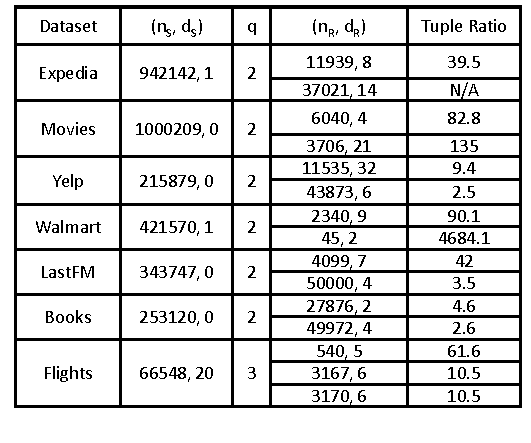
\includegraphics[width=\columnwidth,height=\textheight,keepaspectratio]{table1.pdf}
\caption{Dataset Statistics}
\label{Table:datastats}
\end{table}
We compare \textit{JoinAll} that joins all the base tables with \textit{NoJoin} which avoids all the dimension tables. Each approach is paired with Decision tree (CART) and SVM with RBF kernel based classifier. We compare the total runtime to learn the model and predict the outcome. We have used standard holdout validation method with the fact table split randomly into 50\%:25\%:25\% for training, validation and testing. Since the number of classes in the target for all the 7 datasets is 2, we use zero-one error. 
\begin{table*}
\centering
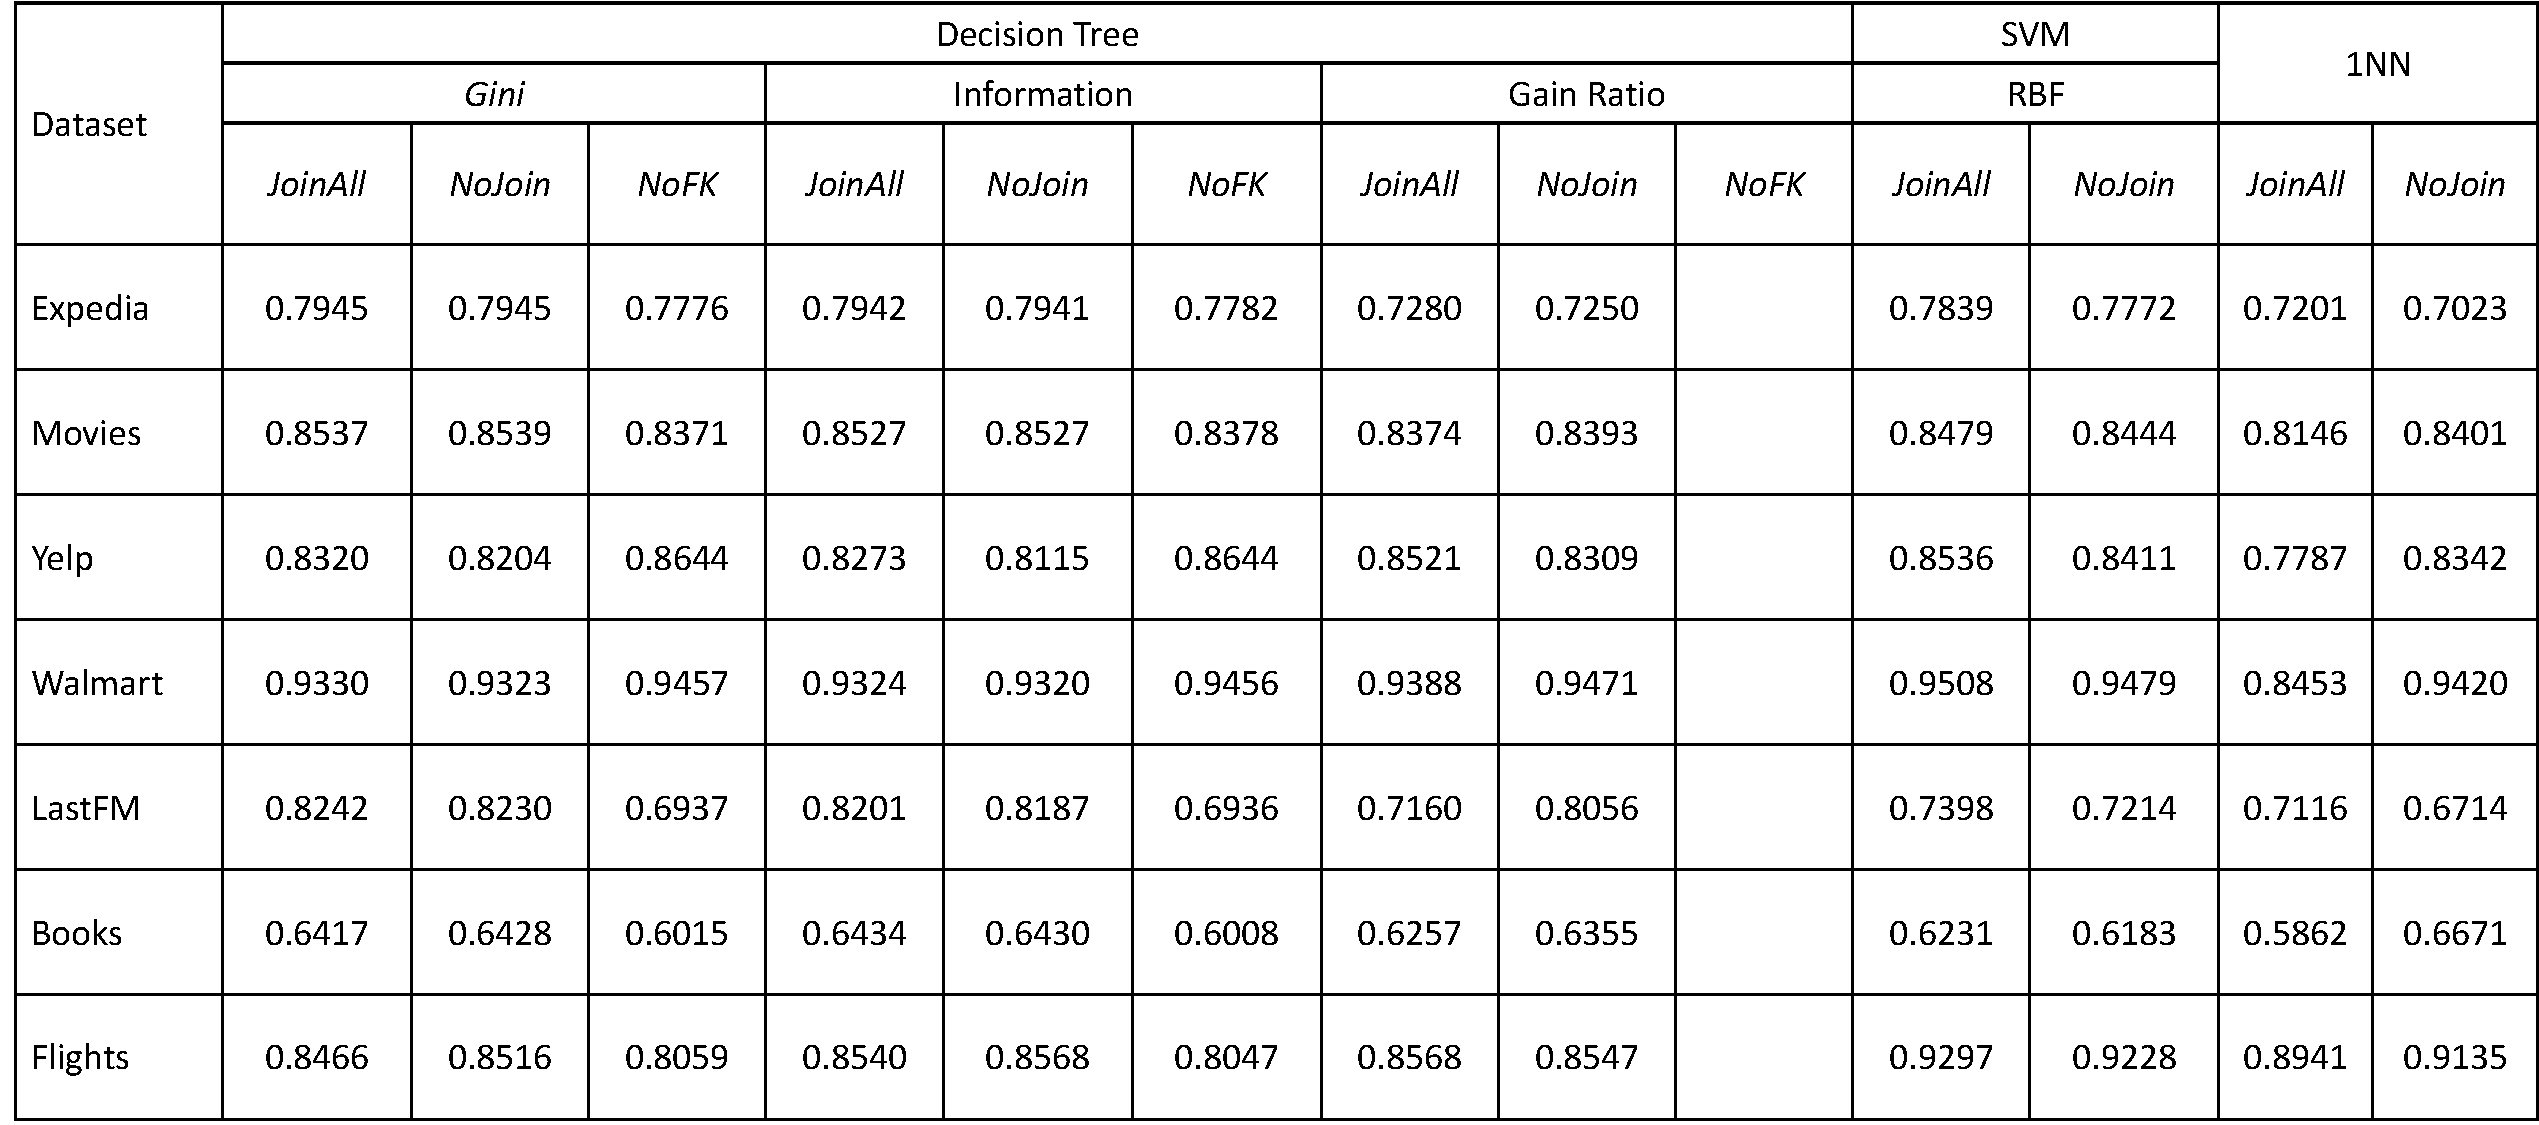
\includegraphics[width=2\columnwidth,height=\textheight,keepaspectratio]{table2.pdf}
\caption{End-to-end results real data}
\label{Table:svm_tree}
\end{table*}
\begin{table*}
\centering
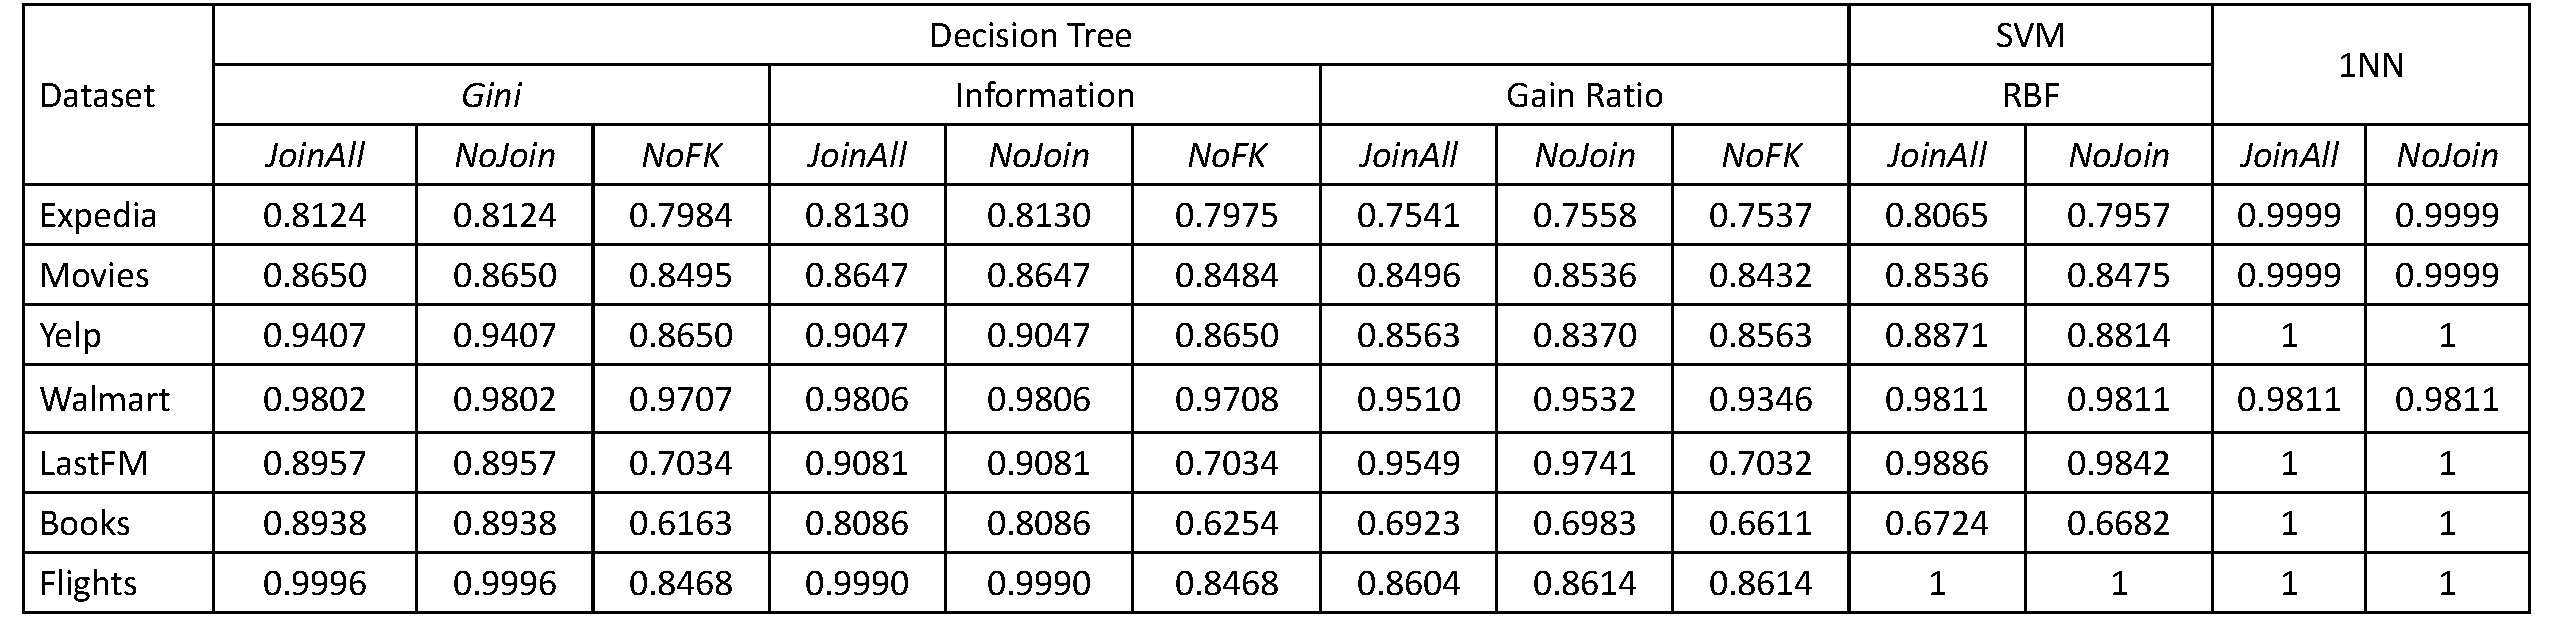
\includegraphics[width=2\columnwidth,height=\textheight,keepaspectratio]{table3.pdf}
\caption{Performance accuracy for training data}
\label{Table:svm_train_tree}
\end{table*}
\begin{table}
\centering
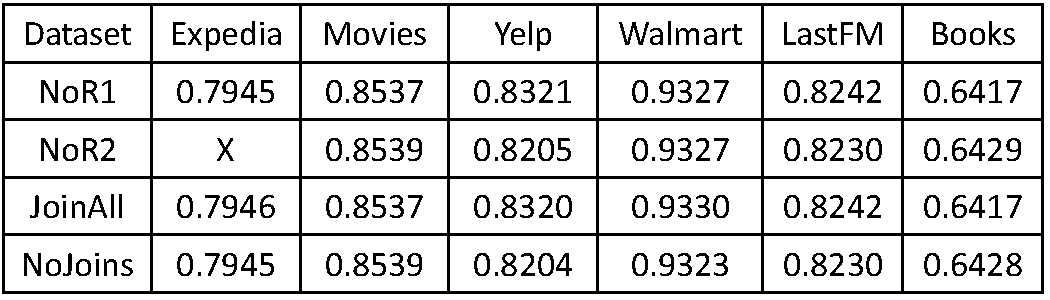
\includegraphics[width=\columnwidth,height=\textheight,keepaspectratio]{table4.pdf}
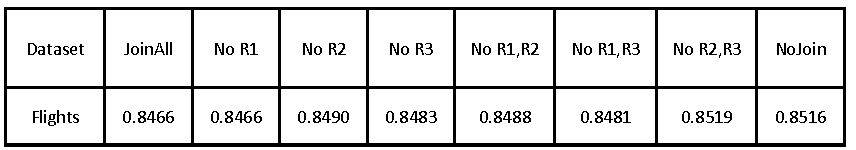
\includegraphics[width=\columnwidth,height=\textheight,keepaspectratio]{table5.pdf}
\caption{Robustness study}
\label{Table:robustness}
\end{table}
\paragraph*{Decision Tree}
In order to evaluate classification performance of the decision tree, we perform a set of 20 cross validation runs using \textit{minsplit} and \textit{cp} as parameters to classify each of the data sets. \textit{minsplit} defines the number of observations that must exist in a node for a split to be attempted and any split that does not improve the fit by a factor of \textit{cp} is pruned off by validation procedure.   
\paragraph*{Gaussian SVM}
For Gaussian SVM we use the e1071 package which is the interface to the popular libsvm libraries. Gaussian SVMs requires tuning two parameters- C and gamma. The parameter C controls the cost of misclassification. A small C(soft margin) makes the cost of misclassification low thus allowing more of data points to lie on the wrong side of the margin. Large C (hard margin) implies high cost of misclassification that can potentially overfit the data. The gamma is a parameter of gaussian kernel given by: \[ k(x_i,x_j) = \exp(-\gamma \cdot \lVert{x_i - x_j} \rVert ^2 ) for \gamma > 0 \].
Where $x_{i}$ and $x_{j}$ are any two data points in the training dataset. A small $\gamma$ implies a gaussian with high variance and vice versa. The parameters C and gamma are determined by searching for maximum accuracy in the 2D-grid formed by different values of C and gamma on the validation set. C was sampled at $10^{-1}$, $10^{0}$, $10^{1}$, $10^{2}$, $10^{3}$ and gamma at $10^{-4}$, $10^{-3}$, $10^{-2}$, $10^{-1}$, $10^{0}$, $10^{1}$. Finally, the accuracies on hold out test data are reported in table\ref{Table:svm_tree}.

\section{In-depth Simulation Study}



\paragraph*{Setup and Data Synthesis}

\begin{figure*}
\centering
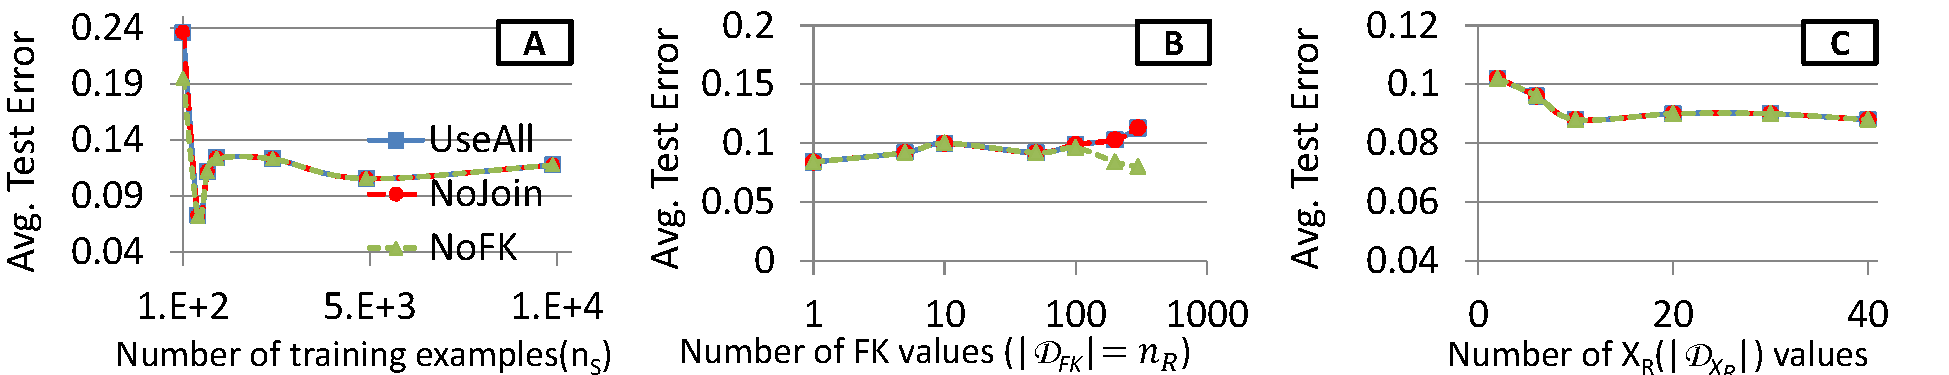
\includegraphics[width=2\columnwidth,height=2\textheight,keepaspectratio]{onexr_row1.pdf}

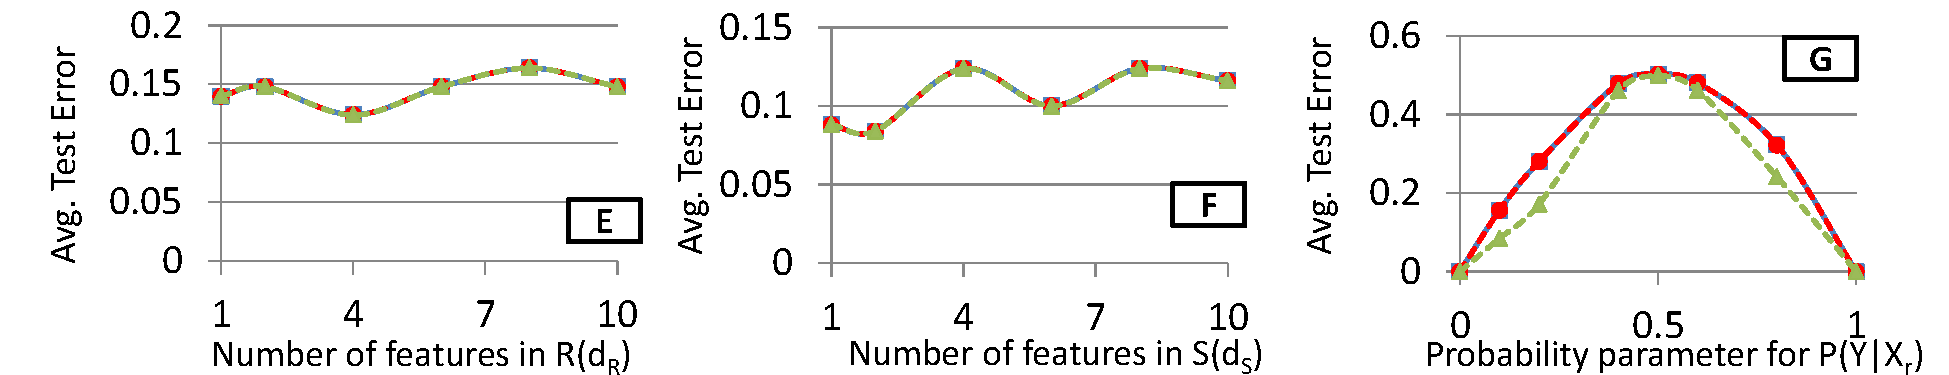
\includegraphics[width=2\columnwidth,height=2\textheight,keepaspectratio]{onexr_row2.pdf}
\caption{OneXr simulation}
\label{Figure:OneXrSimulation}
\end{figure*}
\subsection{Scenario OneXr}

\begin{figure}
\centering
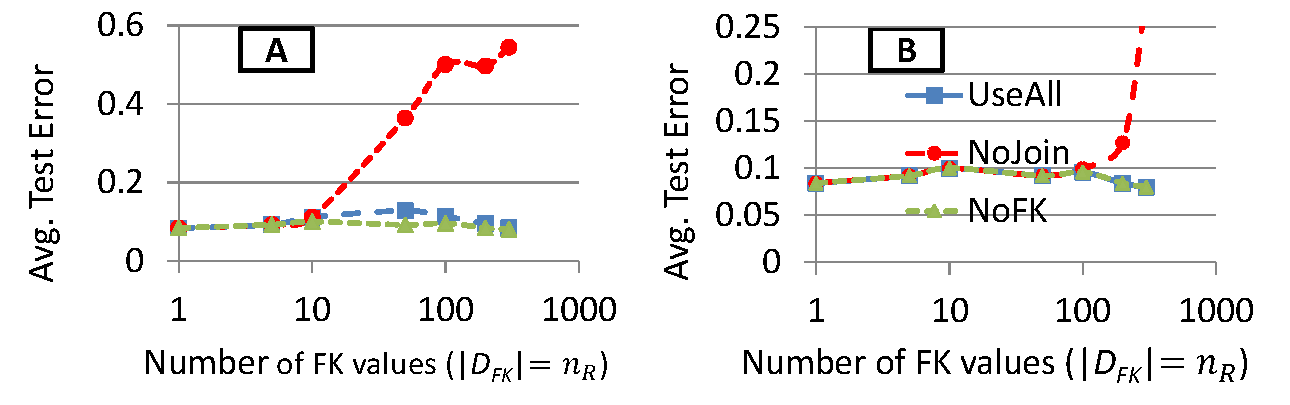
\includegraphics[width=\columnwidth,height=\textheight,keepaspectratio]{onexr_svm_1nn.pdf}
\caption{OneXr simulation for 1nn and SVM}
\label{Figure:OneXr1nnSVMSimulation}
\end{figure}

\begin{figure}
\centering
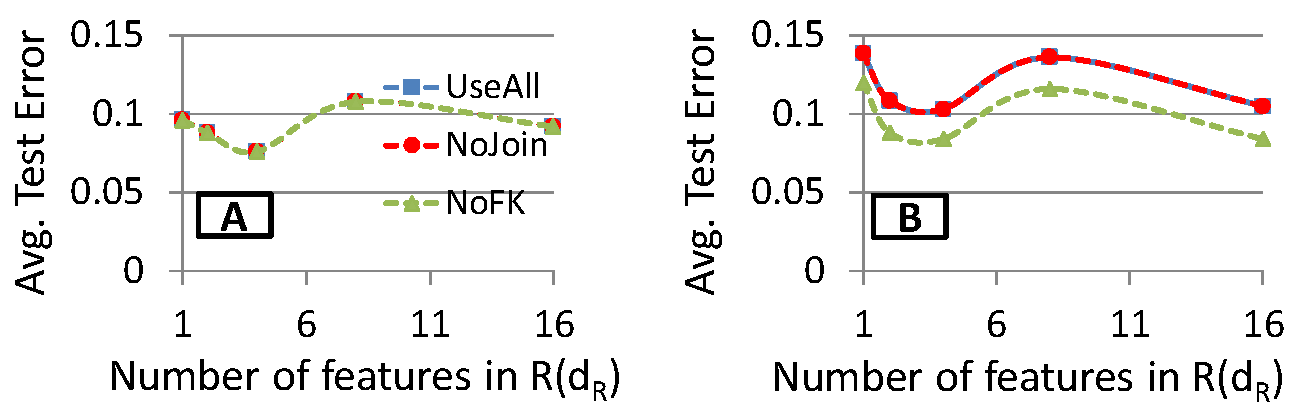
\includegraphics[width=\columnwidth,height=\textheight,keepaspectratio]{onexr_jerrydt.pdf}
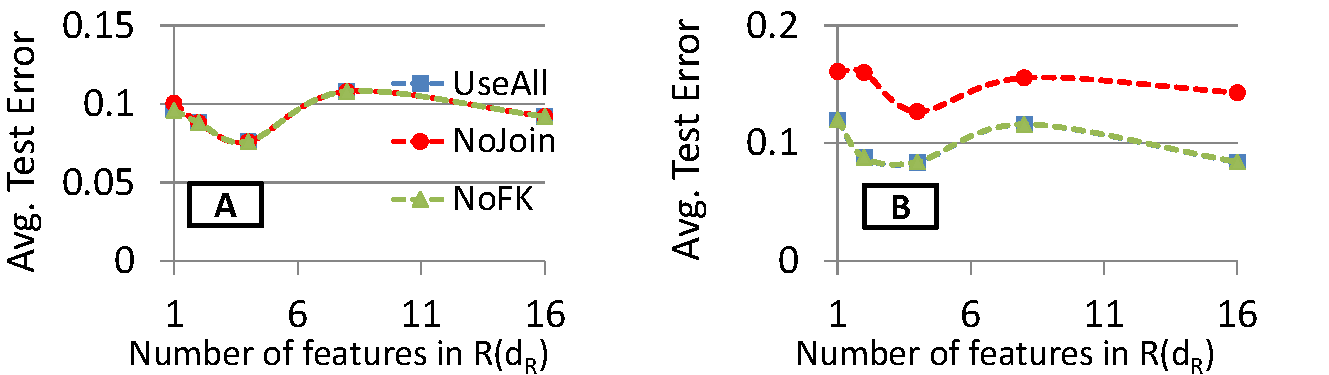
\includegraphics[width=\columnwidth,height=\textheight,keepaspectratio]{onexr_jerrysvm.pdf}
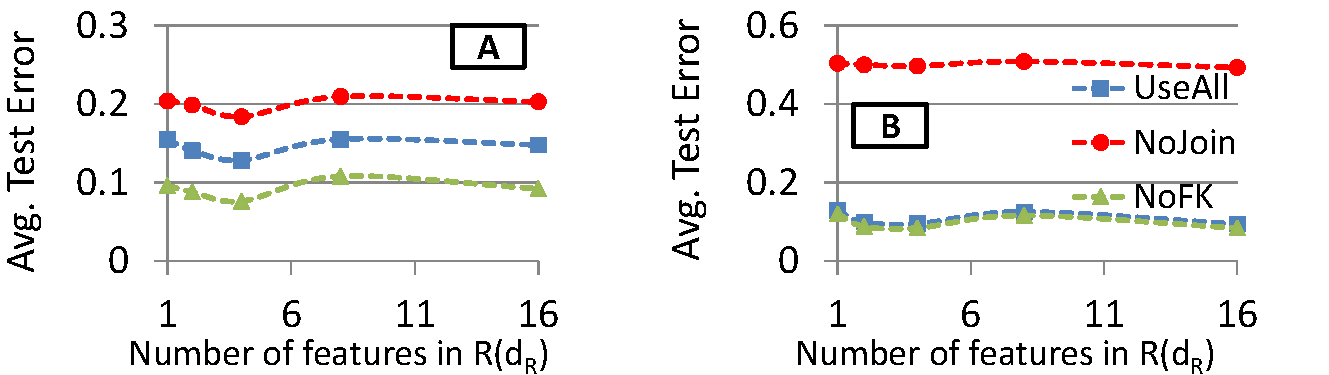
\includegraphics[width=\columnwidth,height=\textheight,keepaspectratio]{onexr_jerry1nn.pdf}
\caption{OneXr simulation for repeated Xr Features}
\label{Figure:OneXrjerry}
\end{figure}


\begin{figure*}
\centering
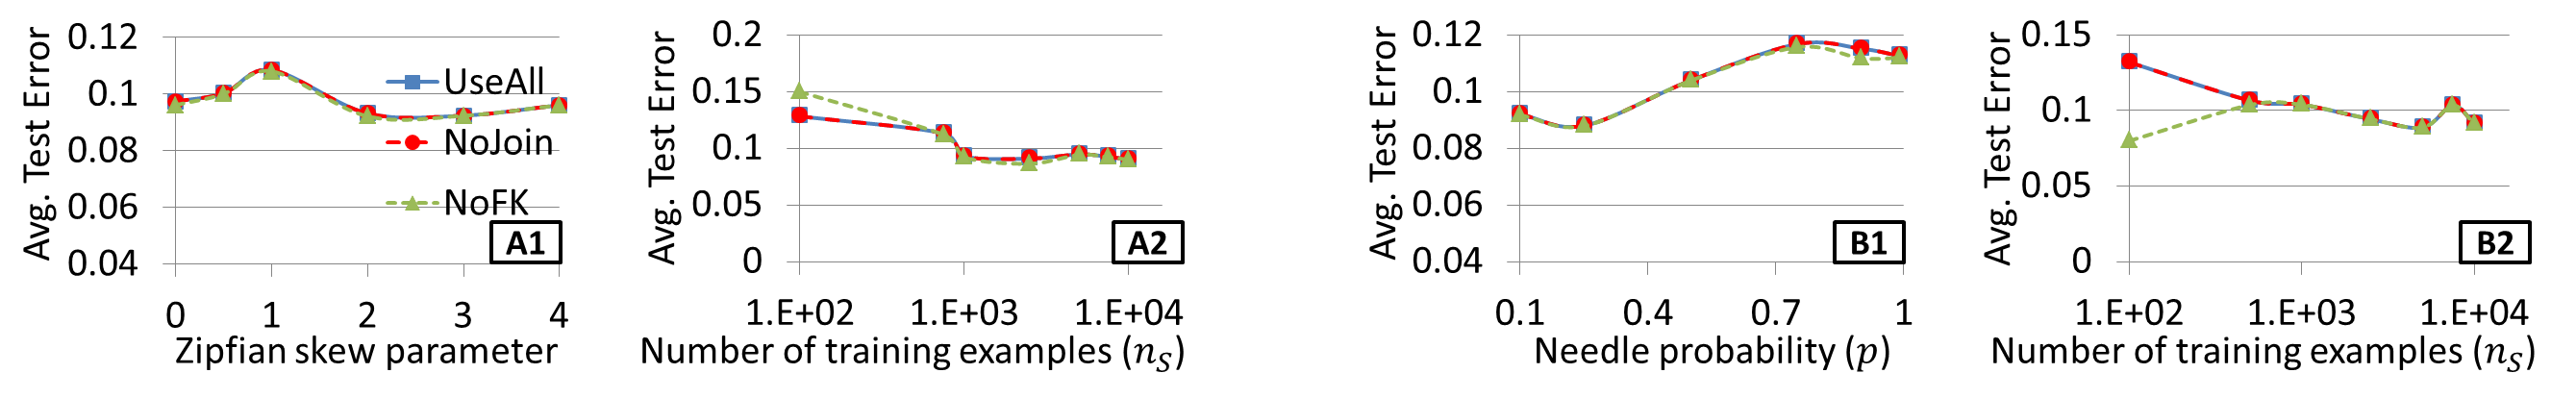
\includegraphics[width=2\columnwidth,height=\textheight,keepaspectratio]{onexr_zipf.png}
\caption{OneXr Zipfian simulation}
\label{Figure:OneXrZipfSimulation}
\end{figure*}


\paragraph*{Scenario SkewedFK}


\subsection{Scenario XSXR}
\begin{figure*}
\centering
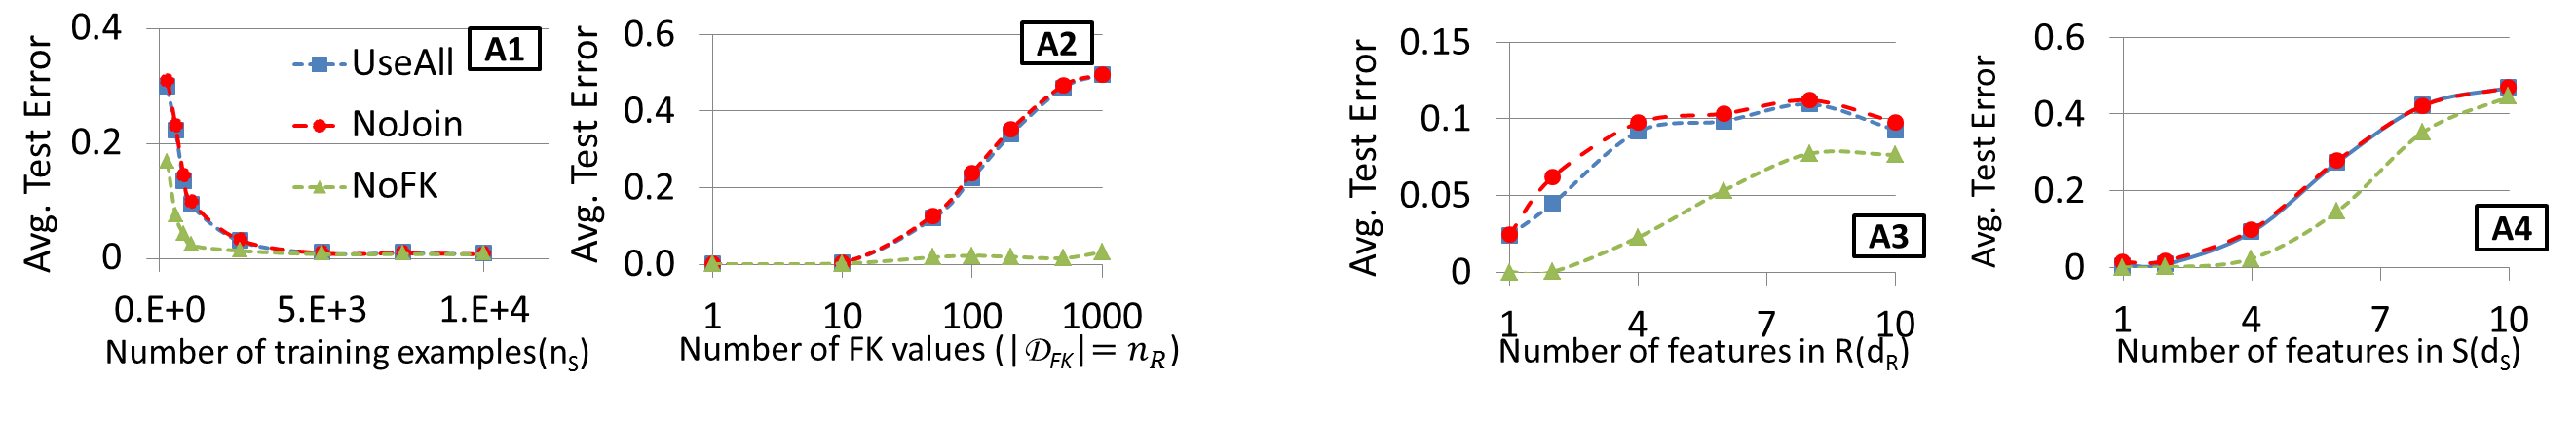
\includegraphics[width=2\columnwidth,height=\textheight,keepaspectratio]{xsxr.png}
\caption{XsXr simulation}
\label{Figure:XsXrSimulation}
\end{figure*}

\subsection{Explanation and Open Questions}

\paragraph*{Decision Tree}

\paragraph*{Gaussian SVM}


\section{Making Foreign Key Features Practical}

\subsection{Foreign Key Domain Compression}

Clearly, foreign keys often act as good representatives of foreign features for \textit{accuracy}.
But they often pose a practical bottleneck for \textit{interpretability} due to the sheer size of their domains.
For example, it is nearly impossible to visualize a decision tree that uses a foreign key feature with 1000s of domain values.
Thus, to make foreign key features more practical, we consider a simple approach: \textit{compress} their domains to a (much) smaller 
user-defined domain size. This is inspired by the hashing trick~\cite{hashingtrick} but instead of an unsupervised random 
compression, we propose a deterministic supervised compression that optimizes some criterion related to accuracy. A key benefit of 
this approach is potentially higher accuracy, while obtaining an interpretable grouping of domain values.
We consider a natural criterion for maximization: \textit{mutual information} of the compressed foreign key with the target.

Formally, given the target $Y$ with domain $\mathcal{D}_Y$, a foreign key feature $FK$ with domain $\mathcal{D}_{FK}$ recoded as $[m]$ 
(where $m = |\mathcal{D}_{FK}|$) and a positive integer ``budget'' $l \ll m$, obtain a mapping $f: [m] \rightarrow [l]$ such that $I(Y; f(FK))$ is maximized,
or equivalently, $H(Y|f(FK))$ is minimized. Essentially, this is a partitioning problem in which we $\mathcal{D}_{FK}$ is partitioned into $l$ subsets. 
We reformulate this as a $0/1$-optimization problem over an $m \times l$ indicator variable matrix $v$.
The input constants are $|\mathcal{D}_Y| \cdot l$ frequency counts of the joint $(Y, FK)$ values in the training dataset, denoted $c_{y, x}$.
The problem then becomes the following:

\begin{equation*}
\begin{aligned}
& \underset{v}{\text{min}}
& & \sum_{y \in \mathcal{D}_Y} \sum_{j=1}^l \bigg(\sum_{i=i}^m c_{y,i} \cdot v_{i,j} \bigg) log \bigg(\frac{\sum_{y' \in \mathcal{D}_Y} \sum_{i=i}^m c_{y,i} \cdot v_{i,j}}{\sum_{i=i}^m c_{y,i} \cdot v_{i,j}}\bigg) \\
& \text{s.t.}
& & \sum_{j=1}^l v_{i,j} = 1, \; i = 1, \ldots, m
\end{aligned}
\end{equation*}

The optimization problem is non-convex and hard to optimize in a brute-force  way due to the number of variables (potentially millions). Thus, we propose two heuristics: \textit{SortBased} and \textit{TreeBased}.

\textit{SortBased} is a greedy approach in which we sort $\mathcal{D}_{FK}$ based on $H(Y|FK=z), ~z \in \mathcal{D}_{FK}$, compute the differences among adjacent pairs of values, and pick the boundaries corresponding to the top $l-1$ differences (ties broken randomly). This gives us an $l$-partition of $\mathcal{D}_{FK}$. The intuition is that by grouping $FK$ values that have comparable conditional entropy values, $H(Y|f(FK))$ is unlikely to increase much compared to $H(Y|FK)$. This approach operates on the training split.

\textit{TreeBased} is a post-hoc approach in which we first learn a decision tree that includes $FK$. Internally, the tree induces a partitioning of 
$\mathcal{D}_{FK}$. We simply construct $f$ using this partitioning information. Let $r$ be the number of subsets of $\mathcal{D}_{FK}$ at the lowest levels of the tree 
(finest-grained partitioning). If $r = l$, each subset directly corresponds to a value in $[l]$. If $r > l$, we use the same greedy approach used for the SortBased 
approach to merge the subsets until we end up with $l$ subsets. Finally, if $r < l$, we simply leave the partitioning as is because we already satisfy the user's budget;
the co-domain of $f$ is then only $[r]$ instead of $[l]$. This approach utilizes both the training and validation splits for learning the best decision tree that includes $FK$, with .

We now empirically compare the accuracy of the above two heuristics against random hashing as a baseline with $l$ as the number of buckets. 
We use the real-world datasets for this experiment and our methodology is as follows. We retain the 50:25:25 train-validate-test split.
\textit{SortBased} and random hashing use just the training split to construct $f$ and then compress $FK$ for the whole dataset. We then use
the validation set as before to tune the hyper-parameters and measure the holdout test error. For random hashing, we report the average across 
five runs. For \textit{TreeBased}, we first learn a decision tree using the original training and validation sets, construct $f$ and compress 
$FK$ for the whole dataset, and then measure the holdout test error.

\begin{figure}
\centering
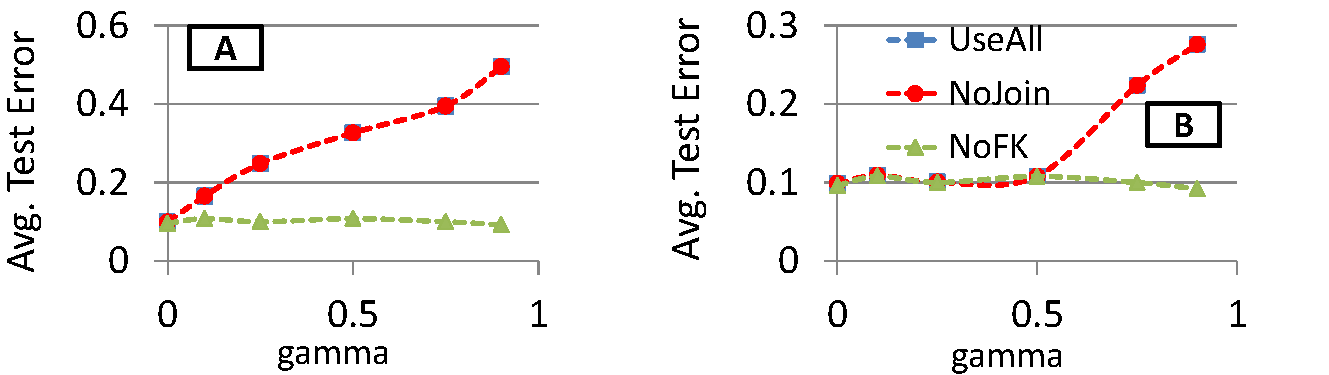
\includegraphics[width=\columnwidth,height=\textheight,keepaspectratio]{smoothing.pdf}
\caption{Smoothing where (A) denotes random based and (B) represents the xr based smoothing}
\label{Figure:OneXr1nnSVMSimulation}
\end{figure}
\subsection{Foreign Key Smoothing}

A closely related issue caused by a large $|\mathcal{D}_{FK}|$ is that some $FK$ values might not be present in the training set but arise 
in the test set or during deployment. Note that this issue is different from the cold start issue because $\mathcal{D}_{FK}$ is still closed 
in this setting. This issue arises because there are simply not enough labeled examples to cover 
all of $\mathcal{D}_{FK}$ during training. Typically, this issue is handled using some form of \textit{smoothing}, e.g., Laplacian smoothing
for Naive Bayes by adding a pseudocount of $1$ to all frequency counts~\cite{mitchellbook}.
While similar smoothing techniques have been studied for probability estimation using decision trees~\cite{pedro2003}, to the best of our knowledge, 
this issue has not been handled in general for classification using decision trees. In fact, popular decision tree implementations in R simply 
crash if a value of $FK$ not seen during training arises during testing! Note that SVMs (or any other classifier operating on numeric 
feature spaces) do not face this issue due to the one-hot recoding of $FK$. 

We consider a simple approach to mitigate this issue: smooth by \textit{reassigning} an $FK$ value not seen during training to an $FK$ value 
seen during training. There are various ways to reassign; for simplicity sake, we only study two lightweight unsupervised methods. 
We use \textit{random} reassignment as a baseline but then study an alternative approach suited to our problem setting: use the foreign features 
($\textbf{X}_R$) to decide the reassignment. This is a natural choice because \textbf{R} provides auxiliary descriptive information about $FK$.
Our algorithm is simple: given a test example with $FK$ not seen during training, obtain an $FK$ seen during training whose corresponding 
$\textbf{X}_R$ feature vector has the minimum $l_0$ distance with the test example's $\textbf{X}_R$ (ties broken randomly). The $l_0$ distance is
simply the count of the number of pairwise mismatches of the respective features in the two $\textbf{X}_R$ feature vectors. 

The intuition for $\textbf{X}_R$-based smoothing is that if $\textbf{X}_R$ is part of the ``true'' distribution, it can provide better accuracy 
than random reassignment. But if $\textbf{X}_R$ is simply noise, it becomes similar to random reassignment.
To demonstrate our point, we now empirically compare their accuracy using our OneXr simulation scenario. Recall that a feature $X_r \in \textbf{X}_R$
determines the target (with some Bayes noise as before). We introduce a parameter $\gamma$ that is the ratio of the number of $FK$ values not seen 
during training to $|\mathcal{D}_{FK}|$. If $\gamma = 0$, no smoothing is needed; as $\gamma$ increases, more smoothing is needed.




\section{Conclusion and Future Work}



\bibliographystyle{ACM-Reference-Format}
\bibliography{MLAvoidJoins}

\end{document}
